
%(BEGIN_QUESTION)
% Copyright 2011, Tony R. Kuphaldt, released under the Creative Commons Attribution License (v 1.0)
% This means you may do almost anything with this work of mine, so long as you give me proper credit

Examine the control solenoids for the backup charge feed pump, which is driven by a steam turbine rather than by an electric motor as is the main charge feed pump:

$$\includegraphics[width=15.5cm]{i0001rx01.eps}$$

The purpose of this backup pump is to turn on automatically if a low pressure condition is sensed at its discharge line, {\it or} turn on manually if an operator actuates a ``hand'' start control.

\vskip 10pt

Label the energized and de-energized flow pathways through each solenoid valve with arrows, assuming the lower solenoid (the one with the reset flag) is normally de-energized and the upper solenoid is normally energized.

\vskip 20pt \vbox{\hrule \hbox{\strut \vrule{} {\bf Suggestions for Socratic discussion} \vrule} \hrule}

\begin{itemize}
\item{} Why do you suppose the backup pump is driven by a steam turbine, while the main pump is driven by an electric motor?  Why not drive both with motors, or both with turbines?
\item{} What is the purpose of having {\it two} low-pressure switches in the auto-start control system rather than a single low-pressure switch?
\end{itemize}

\underbar{file i03432}
%(END_QUESTION)





%(BEGIN_ANSWER)

Incidentally, this is a {\it 1oo2} to trip system, because all it takes is for one of the solenoid valves to trip in order to start up the steam turbine:
 
%(END_ANSWER)





%(BEGIN_NOTES)

$$\includegraphics[width=15.5cm]{i03432x01.eps}$$

\filbreak \vskip 20pt \vbox{\hrule \hbox{\strut \vrule{} {\bf Virtual Troubleshooting} \vrule} \hrule}

\noindent
{\bf Predicting the effect of a given fault:} present each of the following faults to the students, one at a time, having them comment on all the effects each fault would produce.

\begin{itemize}
\item{} 
\item{} 
\item{} 
\end{itemize}


\vskip 10pt


\noindent
{\bf Identifying possible/impossible faults:} present symptoms to the students and then have them determine whether or not a series of suggested faults could account for all the symptoms, explaining {\it why} or {\it why not} for each proposed fault:

\begin{itemize}
\item{} 
\item{} 
\item{} 
\end{itemize}


\vskip 10pt


\noindent
{\bf Determining the utility of given diagnostic tests:} imagine the ??? fails ??? in this system (but don't tell this to students!).  Present the operator's observation(s) to the students, have them consider possible faults and diagnostic strategies, and then propose the following diagnostic tests one by one.  Have students rate the value of each test, determining whether or not each test would give us useful information (i.e. tell us something we don't already know).  Also have students describe what re

\begin{itemize}
\item{} {\it }
\item{}  -- {\bf Yes/No}
\item{}  -- {\bf Yes/No}
\end{itemize}


\vskip 10pt


\noindent
{\bf Diagnosing a fault based on given symptoms:} imagine the SV-142 fails with an electrically open coil.  This causes the turbine to start up, even though pressures are fine and no one commanded it to using HC-142.  Present the operator's observation of a running turbine to the students, have them consider possible faults and diagnostic strategies, and then tell them the results of tests they propose based on the following symptoms, until they have properly identified the nature and location of the fault:

\begin{itemize}
\item{} {\it Turbine is running for no apparent reason}
\item{} IAS at upper solenoid measures 23 PSI
\item{} 122 VAC measured at upper solenoid coil terminals
\item{} 0 VAC measured at lower solenoid coil terminals
\item{} Crack fitting at piston actuator to find no air pressure
\item{} Crack fitting at bottom port of lower solenoid to find no air pressure
\item{} Crack fitting at top port of lower solenoid to find no air pressure
\item{} Crack fitting at bottom port of upper solenoid to find no air pressure
\item{} Crack fitting at top port of upper solenoid to find good air pressure
\item{} PSL-60 status is consistent with adequate pump discharge pressure
\item{} PSL-61 status is consistent with adequate pump discharge pressure
\end{itemize}

%INDEX% Process: distillation, generic (realistic P&ID shown)

%(END_NOTES)


